\newpage
\section{Forward and Inverse Kinematics Analysis: ABB IRB 120}
The task of solving the inverse kinematics for the ABB IRB 120 robot arm is a critical challenge in robotic system design and trajectory planning. Inverse kinematics involves calculating the joint angular positions required to achieve a desired position and orientation of the robot's end-effector. This process is a reverse computation of forward kinematics, where the known joint angles determine the position and orientation of the end-effector. The aim of solving an inverse kinematics solution is to enable the robot arm to interact with its environment in a controlled and predictable manner. This is essential for tasks requiring precision and repeatability. It is also important to note that the solution to the inverse kinematics problem is not unique, meaning that multiple joint configurations can result in the same end-effector position and orientation. Due to its mechanical constraints, the IRB 120 can have up to four different configurations to achieve a targeted end-effector state.

\subsection{Objectives}
\begin{enumerate}
  \item To create a three-dimensional representation of the ABB IRB 120 robot using the Robotics Toolbox for MATLAB\textsuperscript{\textregistered} in the open-source MATLAB\textsuperscript{\textregistered} environment.

  \item To derive and solve the forward and inverse kinematics equations for the ABB IRB 120 robot.

  \item To simulate the robot motion using the Robotics Toolbox for MATLAB\textsuperscript{\textregistered} with the implemented inverse kinematics solutions.
\end{enumerate}

\subsection{Choice of Robot}
For this task, the ABB IRB 120 is used. This robot is known for its compact and agile design, which makes it suitable for a wide range of applications. The IRB 120 is an articulated robot with six degrees of freedom (DOF), allowing for complex movements and high flexibility in task execution.

\noindent The key specifications of the ABB IRB 120 robot are as follows:
\begin{itemize}
  \item \textbf{Degrees of Freedom (DOF):} 6
  \item \textbf{Payload Capacity:} 3 kg
  \item \textbf{Reach:} 580 mm
  \item \textbf{Repeatability:} ±0.01 mm
  \item \textbf{Weight:} 25 kg
  \item \textbf{Wrist Type:} Spherical wrist
\end{itemize}

\noindent The IRB 120's spherical wrist and six axes of movement provides the need for precision in its operation. Its lightweight design, combined with enough payload capacity relative to its size, makes it an ideal choice for educational institutions and learning purposes as well. The robot's dimensions, gotten from the datasheet are as shown below:

\begin{figure}[H]
  \centering
  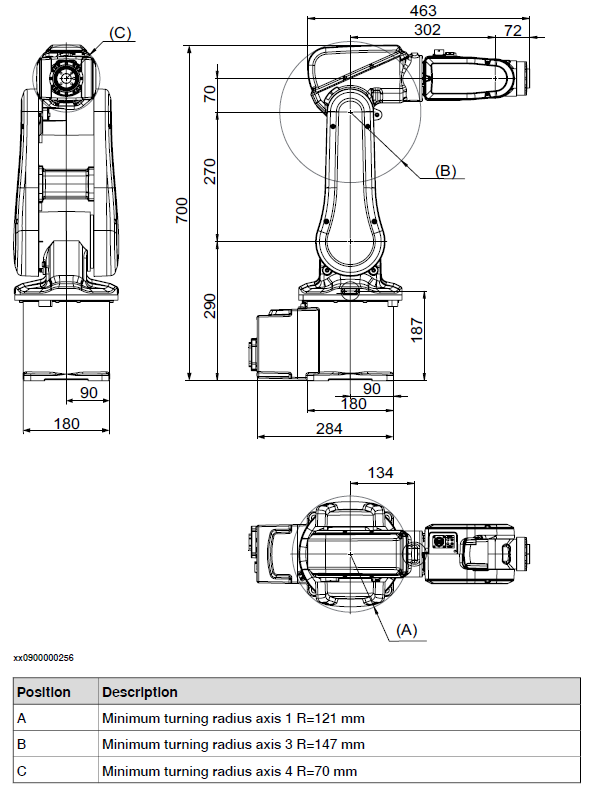
\includegraphics[width=4.8in ]{pics/dimensions_abb.png}
  \caption{ABB IRB 120 Robot Dimensions}\label{dimensions_abb}
\end{figure}


\subsection{Kinematic Representation}

Numerous methods exist for the kinematic representation of robot manipulators, and in this task, we will be using the formulation introduced by Denavit and Hartenberg. The D-H parameters are a set of four values that define the relative position and orientation between adjacent links in a robotic arm. For each joint/link of the robot, the following parameters are assigned:


\begin{itemize}
  \item \textbf{$a_i$:} The distance along the common normal from the z-axis of the previous joint to the z-axis of the current joint.
  \item \textbf{$\alpha_i$:} The angle about the common normal from the z-axis of the previous joint to the z-axis of the current joint. This describes the orientation of one link relative to the previous link.
  \item \textbf{$d_i$:} The offset distance along the previous z-ax s to the common normal, which can vary for prismatic joints.
  \item \textbf{$\theta_i$:} The angle about the previous z-axis from the previous x-axis to the current x-axis, which can vary for revolute joints.
\end{itemize}

\noindent The figure provided below illustrates the established coordinate systems for the Denavit-Hartenberg links as displayed on the manipulator.

\begin{figure}[H]
  \centering
  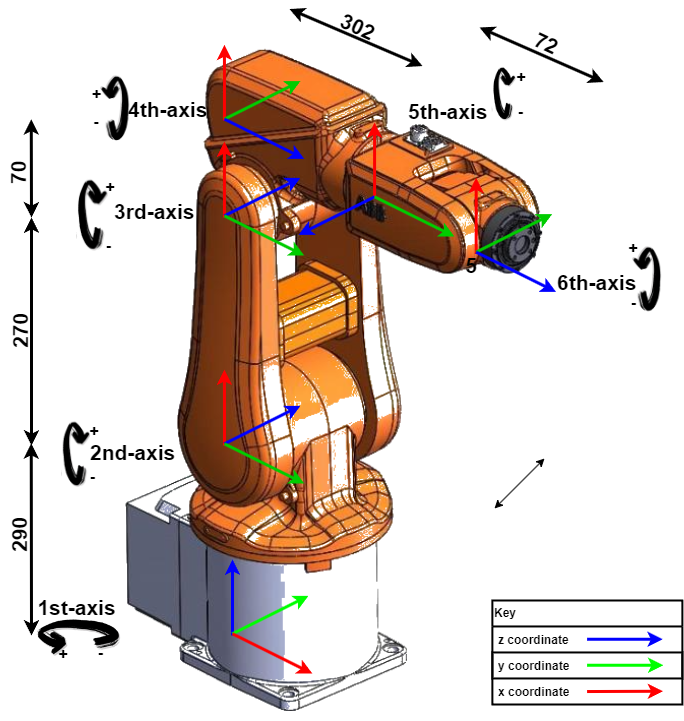
\includegraphics[width=3.6in ]{pics/coordinate frames abb120.drawio.png}
  \caption{ABB IRB 120 Robot with assigned coordinate frames}\label{assigned_coordinates}
\end{figure}


\noindent After defining the coordinate system, the robot’s configuration can be represented using the four D-H parameters explained previously: the joint angle ($\theta_i$), link length ($d_i$), offset distance ($a_i$), and twist angle ($\alpha_i$). Table 1 gives the D-H parameters associated with each link.



% Define the color for the header row
\definecolor{headercolor}{gray}{0}
\renewcommand{\arraystretch}{1.3}

\begin{table}[H]
  \centering\label{tab:dh_parameters}
  \resizebox{0.42\textwidth}{!}{
    \begin{tabular}{|c|c|c|c|}
      \hline
      \rowcolor{headercolor} \color{white}$\theta$ & \color{white}$d$ (mm) & \color{white}$a$ (mm) & \color{white}$\alpha$ (rad) \\
      \hline
      $\theta_1$                                   & 290                   & 0                     & $-\frac{\pi}{2}$            \\
      \hline
      $\theta_2 - \frac{\pi}{2}$                   & 0                     & 270                   & 0                           \\
      \hline
      $\theta_3$                                   & 0                     & 70                    & $-\frac{\pi}{2}$            \\
      \hline
      $\theta_4$                                   & 302                   & 0                     & $\frac{\pi}{2}$             \\
      \hline
      $\theta_5$                                   & 0                     & 0                     & $-\frac{\pi}{2}$            \\
      \hline
      $\theta_6 + {\pi}$                           & 72                    & 0                     & 0                           \\
      \hline
    \end{tabular}
  }
  \caption{DH Parameters of ABB IRB 120}
\end{table}

\noindent
\noindent For a serial-link manipulator with \( n \) joints, the position and orientation of the end-effector with respect to the base frame can be determined by the product of \( n \) homogeneous transformation matrices \( A_i \), each representing the transformation from frame \( i-1 \) to frame \( i \). The transformation matrix for joint \( i \) is given by:
\noindent
\[
  A_i = Rot(z, \theta_i) \cdot Trans(z, d_i) \cdot Trans(x, a_i) \cdot Rot(x, \alpha_i)
\]

where the rotation and translation matrices are defined as:
\noindent
\begin{align*}
  Rot(z, \theta_i) & = \begin{bmatrix}
                         \cos(\theta_i) & -\sin(\theta_i) & 0 & 0 \\
                         \sin(\theta_i) & \cos(\theta_i)  & 0 & 0 \\
                         0              & 0               & 1 & 0 \\
                         0              & 0               & 0 & 1
                       \end{bmatrix}, &
  Trans(z, d_i)    & = \begin{bmatrix}
                         1 & 0 & 0 & 0   \\
                         0 & 1 & 0 & 0   \\
                         0 & 0 & 1 & d_i \\
                         0 & 0 & 0 & 1
                       \end{bmatrix},                          
\end{align*}
\begin{align*}
  Trans(x, a_i)    & = \begin{bmatrix}
                         1 & 0 & 0 & a_i \\
                         0 & 1 & 0 & 0   \\
                         0 & 0 & 1 & 0   \\
                         0 & 0 & 0 & 1
                       \end{bmatrix},                          &
  Rot(x, \alpha_i) & = \begin{bmatrix}
                         1 & 0              & 0               & 0 \\
                         0 & \cos(\alpha_i) & -\sin(\alpha_i) & 0 \\
                         0 & \sin(\alpha_i) & \cos(\alpha_i)  & 0 \\
                         0 & 0              & 0               & 1
                       \end{bmatrix}.
\end{align*}

The final transformation matrix \( A_i \) is given by:
\[
  A_i = \begin{bmatrix}
    \cos(\theta_i) & -\sin(\theta_i)\cos(\alpha_i) & \sin(\theta_i)\sin(\alpha_i)  & a_i\cos(\theta_i) \\
    \sin(\theta_i) & \cos(\theta_i)\cos(\alpha_i)  & -\cos(\theta_i)\sin(\alpha_i) & a_i\sin(\theta_i) \\
    0              & \sin(\alpha_i)                & \cos(\alpha_i)                & d_i               \\
    0              & 0                             & 0                             & 1
  \end{bmatrix}
\]

\noindent The overall transformation matrix \( T \), which describes the pose of the end-effector, is the product of the individual transformation matrices:
\noindent
\[
  T = A_1 A_2 \cdots A_n
\]

\noindent This matrix \( T \) is a \( 4 \times 4 \) homogeneous transformation matrix that contains the position and orientation of the end-effector in its last column and the orientation of the end-effector in the first three columns.


\subsection{Computing Forward Kinematics}
To calculate the forward kinematics of the ABB IRB120 robot, we multiplied all the six A matrices to obtain the final transformation matrix. Alternatively, we used the \texttt{fkine} \cite{RoboticsToolbox} method provided by the Robotics Toolbox for MATLAB\textsuperscript{\textregistered} to confirm if our matrix multiplication was correct and it provided the same values. This method simplifies the process of computing the forward kinematics by taking the joint angles as input and returning the homogeneous transformation matrix representing the pose of the robot's end-effector. Given a set of joint angles, the \texttt{fkine} function computes the position and orientation of the end-effector. By comparing the computed end-effector position \((p_x, p_y, p_z)\) with the position obtained from the RobotStudio\textsuperscript{\textregistered} simulation software (TCP), we can verify the accuracy of our forward kinematics model. If the positions match, it confirms that our forward kinematics computation is correct. The MATLAB\textsuperscript{\textregistered} code for computing the forward kinematics is included in the appendix. After executing the MATLAB\textsuperscript{\textregistered} code, we obtain the position and orientation of the robot's end-effector. The results are then compared with the TCP values from the RobotStudio\textsuperscript{\textregistered} simulation to validate the forward kinematics model. The output from MATLAB\textsuperscript{\textregistered} is as shown below:

\begin{verbatim}
End-effector position: px = -163.9205700, py = -189.00, pz = 711.00
Full Transformation Matrix T:
     0.7704    0.1883   -0.6091    -163.9
    -0.5529    0.6731   -0.4912      -189
     0.3174    0.7152    0.6227       711
          0         0         0         1
\end{verbatim}


\noindent This output can be compared with the end-effector position obtained from the RobotStudio\textsuperscript{\textregistered} simulation, which is given as:

\begin{verbatim}
-162.38 -190.32 711.02
\end{verbatim}

\noindent It is depicted below:

\begin{figure}[H]
  \centering
  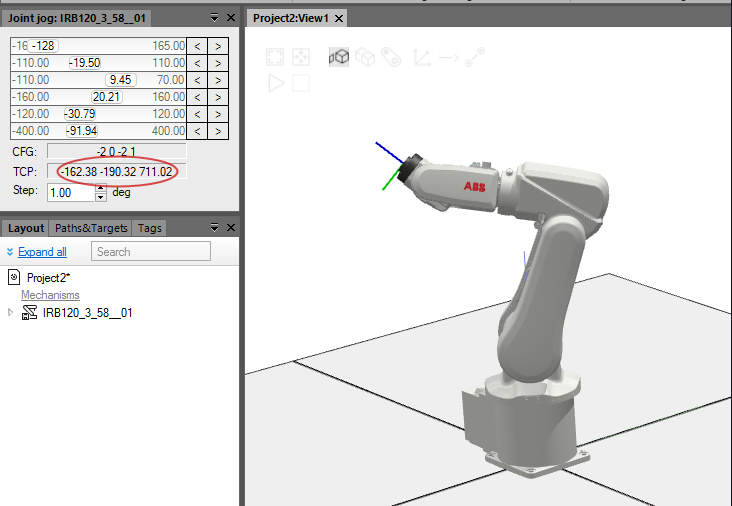
\includegraphics[width=5.2in ]{pics/rstudi.png}
  \caption{Joint Jog interface showing the end-effector position in RobotStudio\textsuperscript{\textregistered}.}\label{joint_jog}
\end{figure}



\noindent Given that the same joint angles are input into both the MATLAB\textsuperscript{\textregistered} function and the RobotStudio\textsuperscript{\textregistered} simulation, we can calculate the percentage error for the end-effector position coordinates to assess the accuracy of the forward kinematics model. The percentage error for each coordinate is calculated as follows:

\[
  \text{Percentage Error} = \left| \frac{\text{Actual Value} - \text{Simulated Value}}{\text{Simulated Value}} \right| \times 100
\]
\\
For the \( p_x \), \( p_y \), and \( p_z \) coordinates, the percentage errors are:

\[
  \text{Percentage Error}_{p_x} = \left| \frac{-163.92 - (-162.38)}{-162.38} \right| \times 100 \approx 0.95\%
\]
\[
  \text{Percentage Error}_{p_y} = \left| \frac{-189.00 - (-190.32)}{-190.32} \right| \times 100 \approx 0.69\%
\]
\[
  \text{Percentage Error}_{p_z} = \left| \frac{711.00 - 711.02}{711.02} \right| \times 100 \approx 0.0028\%
\]
\noindent
\noindent The slight differences observed between the MATLAB\textsuperscript{\textregistered} output and the RobotStudio\textsuperscript{\textregistered} simulation can be attributed to various factors, including numerical rounding errors in the computation, differences in the internal representation of joint angles, or slight variations in the robot model used in the simulation compared to the theoretical model used in the MATLAB\textsuperscript{\textregistered} computation.

\begin{table}[H]
  \centering\label{tab:percentage_error}
  \begin{tabular}{|c|c|c|}
    \hline
    \rowcolor{black} \color{white}Coordinate & \color{white}MATLAB Value & \color{white}Percentage Error \\
    \hline
    \( p_x \)                                & -163.92                   & 0.95\%                        \\
    \hline
    \( p_y \)                                & -189.00                   & 0.69\%                        \\
    \hline
    \( p_z \)                                & 711.00                    & 0.0028\%                      \\
    \hline
  \end{tabular}
  \caption{Percentage Error in End-Effector Position}
\end{table}


\newpage
\subsection{Inverse Kinematics}
Inverse kinematics for the ABB IRB 120 robot, which has six degrees of freedom (DOF) with all revolute joints and a spherical wrist, can be efficiently solved using the kinematic decoupling approach as described by Seth Hutchinson and Mark W. Spong in \textit{Robot Modeling and Control} \cite{Modeling}. This approach simplifies the complex inverse kinematics problem into two manageable sub-problems: inverse position kinematics and inverse orientation kinematics \cite{Modeling}.

\subsubsection{Kinematic Decoupling}
The kinematic decoupling method is particularly useful for manipulators with six joints where the last three joint axes intersect at a common point, forming a spherical wrist \cite{Modeling}. Other types of robot manipulators can also have a spherical wrist in different setups like RPP + Spherical Wrist (R for Revolute, P for Planar), RRP Spherical Manipulator and so on. This allows the inverse kinematics problem to be divided into finding the position of the wrist center and determining the orientation of the wrist.

\noindent For a six-DOF manipulator with a spherical wrist, the inverse kinematics can be broken into two steps:

\begin{enumerate}
  \item  \textbf{Position problem:} Finding the position of the wrist center (\(\theta_1\)\(\theta_2\)\(\theta_3\)).
  \item  \textbf{Orientation problem}: Determining the orientation of the wrist (\(\theta_4\)\(\theta_5\)\(\theta_6\)).
\end{enumerate}


\begin  {figure}[H]
\centering
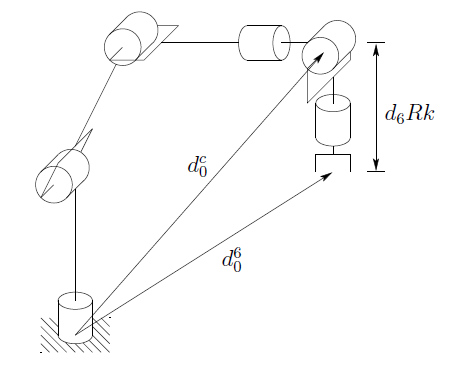
\includegraphics[width=3.5in]{pics/inverse_hutchinson.png}
\caption {Illustration of Kinematic Decoupling \cite{Modeling}}
\label{fig:kinematic_decoupling}
\end{figure}

\subsubsection{Determining Origin of Spherical Wrist}
So we will start our workings from the wrist centre, but the problem is we do not know where the wrist centre is, in terms of its coordinates / location. To find the location of the origin of the wrist, we will come back from the end effector (Joint 6) and offset by \(z_6\) to get to wrist position origin.
\noindent This offset is 72 mm along the \(Z_6\) direction, and we use the last column of the rotation matrix to represent \(Z_6\) in the base frame. By subtracting this offset, we obtain the wrist center position (\(\mathbf{o}_c^0\)):

\[
  \mathbf{o}_c^0 = \mathbf{o}_6^0 - d_6 \mathbf{z}_6^0 = \mathbf{o}_6^0 -72{R}_6^0
\]

\noindent where \(\mathbf{o}_c^0\) is the end-effector position, \(d_6\) is the offset distance 72 mm, \(\mathbf{o}_6^0\) is the \((p_x, p_y, p_z)\) of the final transformation matrix, and \(\mathbf{R}_6^0\) is the unit vector along \(Z_6\). To understand this better, this can be represented in component form as follows:

\[
  \begin{pmatrix}
    x_c \\
    y_c \\
    z_c
  \end{pmatrix} =
  \begin{pmatrix}
    o_x \\
    o_y \\
    o_z
  \end{pmatrix} -
  d_6
  \begin{pmatrix}
    r_{13} \\
    r_{23} \\
    r_{33}
  \end{pmatrix}
\]

\noindent where \(p_x\), \(p_y\), and \(p_z\) are the components of the desired end-effector position, and \(r_{13}\), \(r_{23}\), and \(r_{33}\) are the elements of the third column of the rotation matrix \(\mathbf{R}\). This can be seen in the rough sketch below.

\begin{figure}[H]
  \centering
  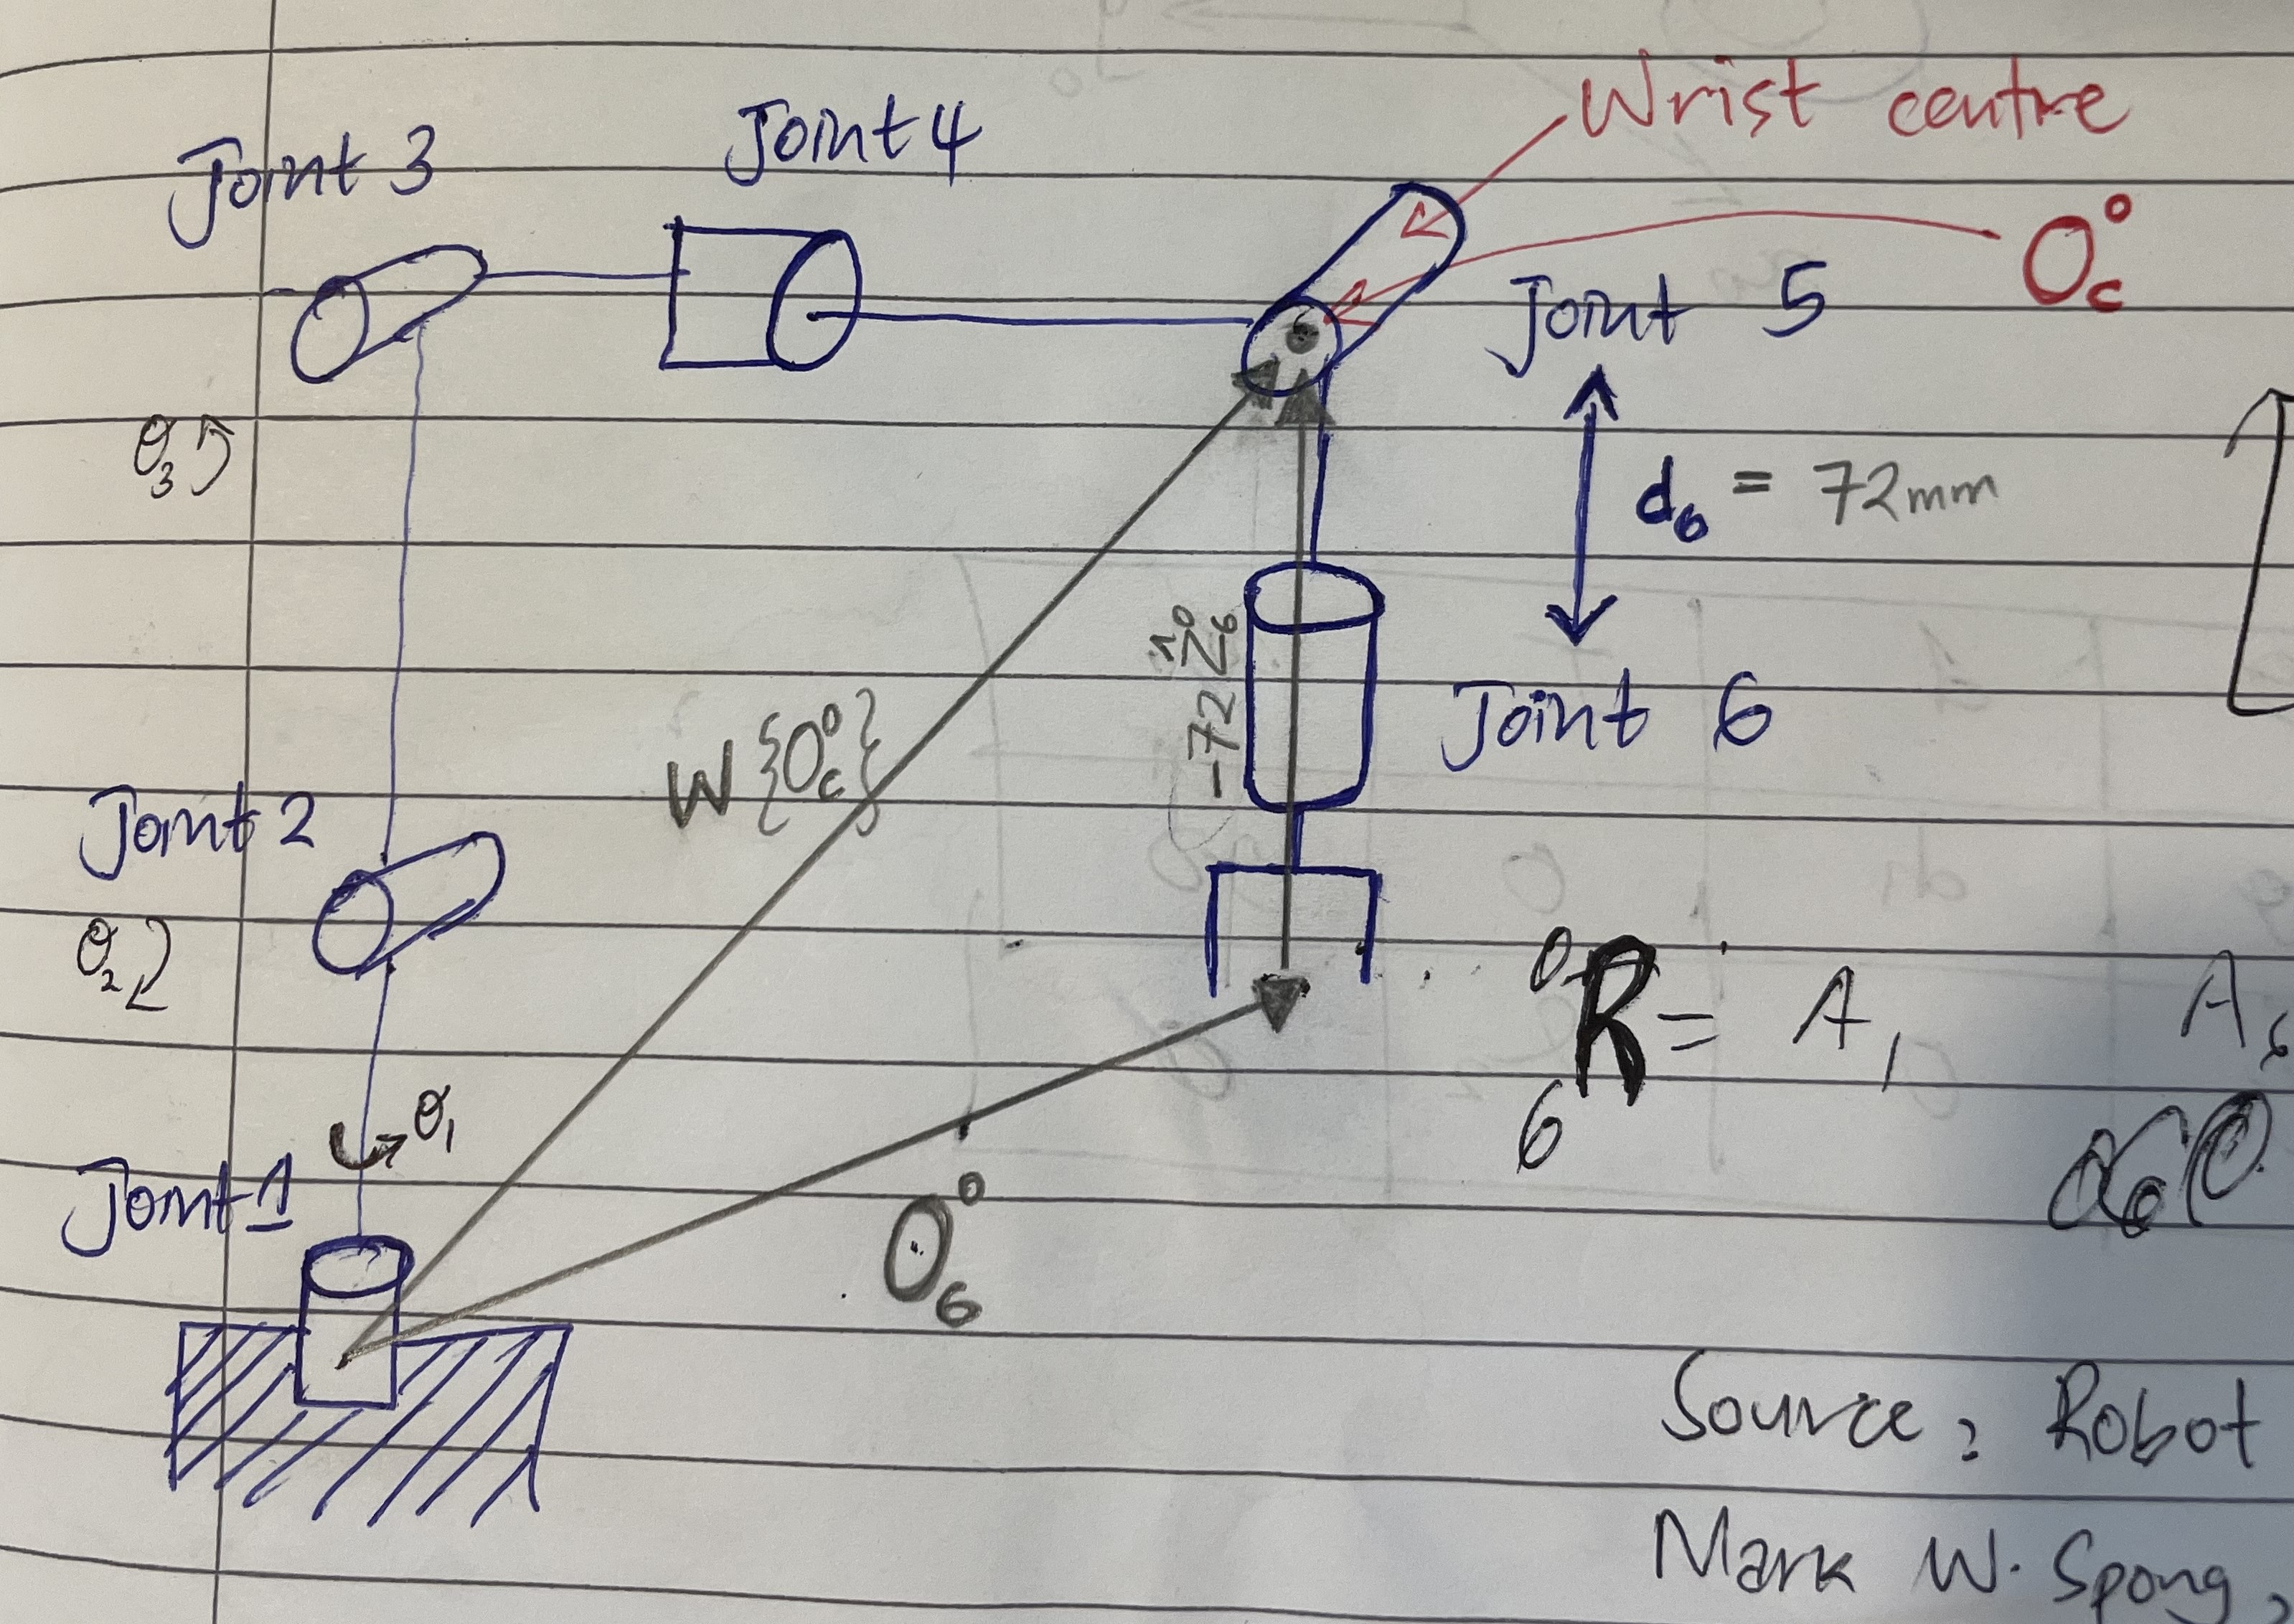
\includegraphics[width=4.0in ]{pics/decoup_sketch.JPG}
  \caption{Sketch of spherical wrist .}
  \label{sphericalw}
\end{figure}


\noindent Next, we define the transformation matrices (\(A_1\) to \(A_6\)) for each joint using the DH parameter. These will be the inputs for the orientation of the object when we finally solve the inverse kinematics and have to input the position and orientation of the object to find the joint angles. In the MATLAB\textsuperscript{\textregistered} code, this is implemented here:

\begin{lstlisting}[frame=single,style=Matlab-Pyglike]
% Prompt for end effector position and orientation
O60 = input('Enter the end effector position as a 3-element vector [x; y; z]: ');
R60 = input('Enter the end effector orientation as a 3x3 rotation matrix: ');
Oc0 = O60 - 72 * R60(:,3);   % wrist position
\end{lstlisting}




\subsubsection{Determining Position of Wrist \texorpdfstring{$\left(p_x, p_y, p_z\right)$}{px, py, pz} of \texorpdfstring{$\left(\mathbf{T}_4^0\right)$}{T40}}

The location of the wrist depends only on \(\theta_1\), \(\theta_2\), and \(\theta_3\). \(\theta_4\) only accounts for the distance 302 mm because it rotates about axis \(Z_3\), which doesn’t change the position of the point.. So this means that we will only consider the transformation matrix from the DH parameters until the fourth A matrix.

\[
  T_4^0 = A_1 \cdot A_2 \cdot A_3 \cdot A_4
\]

\noindent In the MATLAB code, the function  this is implemented here:

\begin{lstlisting}[frame=single,style=Matlab-editor]
T40 = A1*A2*A3*A4;

disp('Wrist position (considered upto link 4)');
wp = simplify(T40(1:3,4));  % last column, px py pz
disp(wp)
\end{lstlisting}


\subsubsection{Determining \texorpdfstring{$\theta_1$, $\theta_2$, and $\theta_3$}{theta1, theta2, and theta3}}

\noindent After having determined the wrist center position from MATLAB, \(T_4^0\), it is given by:

\[
  \left(\begin{array}{c}
      2\,\cos \left(\theta_1 \right)\,{\left(151\,\cos \left(\theta_2 +\theta_3 \right)+35\,\sin \left(\theta_2 +\theta_3 \right)+135\,\sin \left(\theta_2 \right)\right)} \\
      2\,\sin \left(\theta_1 \right)\,{\left(151\,\cos \left(\theta_2 +\theta_3 \right)+35\,\sin \left(\theta_2 +\theta_3 \right)+135\,\sin \left(\theta_2 \right)\right)} \\
      270\,\cos \left(\theta_2 \right)+2\,\sqrt{24026}\,\cos \left(\theta_2 +\theta_3 +\mathrm{atan}\left(\frac{151}{35}\right)\right)+290
    \end{array}\right)
\]

\noindent Since the position depends only on \(\theta_1\), \(\theta_2\), and \(\theta_3\), we can solve for these angles.

\noindent For \(\theta_1\):

The wrist center's \(x\) and \(y\) coordinates can be written as:
\[
  p_x = 2\,\cos(\theta_1)\,k
\]
\[
  p_y = 2\,\sin(\theta_1)\,k
\]

where
\[
  k = 151\,\cos(\theta_2 + \theta_3) + 35\,\sin(\theta_2 + \theta_3) + 135\,\sin(\theta_2)
\]

By eliminating \(k\), we have:
\[
  \tan(\theta_1) = \frac{p_y}{p_x}
\]

\begin{center}
  \shadowbox{
    \(\theta_1 = \tan^{-1}\left(\frac{p_y}{p_x}\right)
    \)
  }
\end{center}


\noindent For \(\theta_2\) and \(\theta_3\), using trigonometric identities:
\[
  \sin(\theta_1)\cos(\theta_2) + C_1\sin(\theta_2) = S_{12}
\]
\[
  \cos(\theta_1)\cos(\theta_2) - S_1\sin(\theta_2) = C_{12}
\]

where \(C_1 = \cos(\theta_1)\), \(S_1 = \sin(\theta_1)\), \(C_{12} = \cos(\theta_2 + \theta_3)\), and \(S_{12} = \sin(\theta_2 + \theta_3)\).

\noindent Simplifying the \(z\)-coordinate of the wrist position:
\[
  p_z = 270\,\cos(\theta_2) + 2\,\sqrt{24026}\,\cos\left(\theta_2 + \theta_3 + \mathrm{atan}\left(\frac{151}{35}\right)\right) + 290
\]




Using the trigonometric identity:
\[
  \cos(a + b) = \cos(a)\cos(b) - \sin(a)\sin(b)
\]

we can solve for \(\theta_2\) and \(\theta_3\) by substituting and simplifying the equations.

\noindent Since \(\tan (\beta) = \frac{151}{35}\), we look for \(\cos (\beta)\) and \(\sin (\beta)\)

Using Pythagoras' theorem,
\[
  a^2 + b^2 = c^2
\]
\[
  \tan^{-1}(\theta) = \frac{a}{b} \implies \cos (\theta) = \frac{a}{c}
\]
\[
  c^2 = \sqrt{a^2 + b^2}
\]

In tangent, \(c = \frac{a}{\tan (\theta)}\)
\[
  a^2 = (c \cdot \tan (\theta))^2
\]
\[
  c^2 = a^2 + (a \cdot \tan (\theta))^2
\]
\[
  c = a \sqrt{1 + \tan^2 (\theta)}
\]
\[
  a = \frac{c}{\sqrt{1 + \tan^2 (\theta)}}
\]

So \(\cos (\beta)\) is:
\[
  \cos (\beta) = \frac{1}{\sqrt{1 + \tan^2 (\beta)}} = \frac{1}{\sqrt{1 + \left( \frac{151}{35} \right)^2}} = \frac{1}{\sqrt{1 + \frac{22801}{1225}}} = \frac{1}{\sqrt{\frac{24026}{1225}}} = \frac{\sqrt{1225}}{\sqrt{24026}} = \frac{35}{\sqrt{24026}}
\]





\[
  \sin (\beta) = \cos (\beta) \cdot \tan (\beta) = \frac{35}{\sqrt{24026}} \cdot \frac{151}{35} = \frac{151}{\sqrt{24026}}
\]

So,
\[
  \cos (\theta_2 + \theta_3 + \beta) = \cos (\theta_2 + \theta_3) \frac{35}{\sqrt{24026}} - \sin (\theta_2 + \theta_3) \frac{151}{\sqrt{24026}}
\]

\[
  270 \cos (\theta_2) + 2 \sqrt{24026} \cdot \left[ \cos (\theta_2 + \theta_3) \frac{35}{\sqrt{24026}} - \sin (\theta_2 + \theta_3) \frac{151}{\sqrt{24026}} \right] + 290
\]

\[
  = 270 \cos (\theta_2) + 70 \cos (\theta_2 + \theta_3) - 302 \sin (\theta_2 + \theta_3) + 290
\]

\noindent Wrist position with Trigonometry simplification:
\[
  \begin{aligned}
    C_1 (302 \cos (\theta_3) + 70 \sin (\theta_2 + \theta_3) + 270 \sin (\theta_2))            & = X_c       \\
    S_1 (302 \cos (\theta_3) + 70 \sin (\theta_2 + \theta_3) + 270 \sin (\theta_2))            & = Y_c       \\
    270 \cos (\theta_2) + 70 \cos (\theta_2 + \theta_3) - 302 \sin (\theta_2 + \theta_3) + 290 & = Z_c - 290
  \end{aligned}
\]



\noindent Square the 3 equations to eliminate \( \theta_1 \), i.e., \( C_1 \) and \( S_1 \)

\begin{align*}
   & X_c^2 + Y_c^2 + (Z_c - 290)^2 = (302 \cos (\theta_3) + 70 \sin (\theta_2 + \theta_3) + 270 \sin (\theta_2))^2 \\
   & + (270 \cos (\theta_2) + 70 \cos (\theta_2 + \theta_3) - 302 \sin (\theta_2 + \theta_3))^2
\end{align*}


Assuming it's a quadratic equation:
\[
  \frac{-b \pm \sqrt{b^2 - 4ac}}{2a}
\]

Substitute \(S_3\) into the equation:
\[
  C = A \cdot C_3 + B \cdot \sqrt{1 - C_3^2}
\]

\[
  C^2 = (A \cdot C_3)^2 + (B \cdot \sqrt{1 - C_3^2})^2
\]

\[
  (A^2 + B^2) \cdot C_3^2 - 2AC \cdot C_3 + (C^2 - B^2) = 0
\]

\[
  \theta_3 = \cos^{-1} \left( \text{roots} \left( [A^2 + B^2, -2AC, C^2 - B^2] \right) \right)
\]

\noindent To solve for \(\theta_3\), we can use either the \(\cos^{-1}\) function or the \(\tan^{-1}\) function. The possible solutions for \(\theta_3\) are given by:

\begin{center}
  \shadowbox{
    \(\theta_3 = \cos^{-1} \left( \text{roots} \left( [A^2 + B^2, -2AC, C^2 - B^2] \right) \right)\)
  }
\end{center}


\noindent or using the \(\tan^{-1}\) function:

\begin{center}
  \shadowbox{
    \(\theta_3 = \tan^{-1} \left( \sqrt{1 - D(1)^2}, D(1) \right)\)
  }
\end{center}



\noindent The MATLAB\textsuperscript{\textregistered} code for finding \(\theta_3\) is as follows:
\begin{lstlisting}[frame=single,style=Matlab-editor]
% three equations from wrist position
A = 2 * (270^2);
B = 2 * 70 * 302 * 270;
% B=2*70*270;
%B=2*70*302;  % correct one
C = xc^2 + yc^2 + (zc - 290)^2 - 302^2 - 70^2 -270^2;
% D=acos(roots([A^2+B^2,-2*A*C,C^2-B^2]));
D = roots([A^2 + B^2, -2 * A * C, C^2 - B^2]);

% theta3 = D(1);
theta3 = atan2(sqrt(1 - D(1)^2), D(1));
\end{lstlisting}

\subsubsection{Calculating \texorpdfstring{$\theta_2$}{theta2}}

Once \(\theta_3\) is known, we factor out the coefficients of \(\theta_2\) from equation (3):
\[
  270C_2 + 70C_{23} - 302S_{23} = Z_c - 290 \\
\]
\noindent
\[
  C_2 \left( 270 + 70 C_3 - 302 S_3 \right) + S_2 \left( -70 S_3 + 302 C_3 \right) = Z_c - 290
\]


\noindent We can solve for \(\theta_2\) by forming a quadratic equation:
\[
  C_2 \left( 270 + 70 C_3 - 302 S_3 \right) + S_2 \left( -70 S_3 + 302 C_3 \right) = Z_c - 290
\]

The solution for \(\theta_2\) in terms of the MATLAB code is obtained as follows:

\begin{center}
  \shadowbox{
    \(\theta_2 = \mathrm{atan2}\left(-\sqrt{1 - D_2^2}, D_2\right)\)
  }
\end{center}
where \( D_2 \) is obtained from solving the quadratic equation:
\[
  AA^2 + BB^2, -2AA \cdot CC, CC^2 - BB^2
\]
with:
\[
  AA = 270 + 70 \cos(\theta_3) - 302 \sin(\theta_3)
\]
\[
  BB = -70 \sin(\theta_3) - 302 \cos(\theta_3)
\]
\[
  CC = Z_c - 290
\]

The value of \(\theta_2\) is then converted to degrees:
\[
  \theta_2^{\text{deg}} = \text{rad2deg}(\theta_2)
\]


\noindent The MATLAB\textsuperscript{\textregistered} code for solving \(\theta_2\) is as follows:
\begin{lstlisting}[frame=single,style=Matlab-editor]
AA = 270 + 70 * cos(theta3) - 302 * sin(theta3);
BB = -70 * sin(theta3) - 302 * cos(theta3);
CC = zc - 290;

% Solve the quadratic equation
DD = real(roots([AA^2 + BB^2, -2*AA*CC, CC^2 - BB^2]));
theta2 = real(atan2(-sqrt(1 - DD(2)^2), DD(2)));
theta2_deg = rad2deg(theta2);
fprintf('theta2 = %.3f radians, %.3f degrees\n', theta2, theta2_deg);
\end{lstlisting}





\begin{table}[H]
  \centering
  \begin{tabular}{|c|c|c|c|}
    \hline
    \(\theta\)                   & \(d\) (mm) & \(a\) (mm) & \(\alpha\) (rad)   \\
    \hline
    \(\theta_1\)                 & 290        & 0          & \(-\frac{\pi}{2}\) \\
    \hline
    \(\theta_2 - \frac{\pi}{2}\) & 0          & 270        & 0                  \\
    \hline
    \(\theta_3\)                 & 0          & 70         & \(-\frac{\pi}{2}\) \\
    \hline
    \(\theta_4\)                 & 302        & 0          & \(\frac{\pi}{2}\)  \\
    \hline
    \(\theta_5\)                 & 0          & 0          & \(-\frac{\pi}{2}\) \\
    \hline
    \(\theta_6 + \pi\)           & 72         & 0          & 0                  \\
    \hline
  \end{tabular}
  \caption{DH Parameters of ABB IRB 120}
\end{table}

\noindent We then multiply these matrices to get the forward kinematics transformation from the base frame to the end-effector (\(T_6^0\)). We also compute the transformation matrices up to the wrist (\(T_4^0\)), which we use to find the wrist position in terms of the first three joint angles.



\[
  T_6^0 = A_1 A_2 A_3 A_4 A_5 A_6
\]

\noindent By computing the transformation matrices up to the wrist center (\(T_4^0\)), we find the position of the wrist center in terms of \(\theta_1\), \(\theta_2\), and \(\theta_3\).


\subsubsection{Determining \texorpdfstring{$\theta_4$, $\theta_5$, and $\theta_6$}{theta4, theta5, and theta6}}

From the given rotation matrix:
\[
  R_6^0 = R_3^0 R_6^3
\]

\noindent where \(\mathbf{R}_0^3\) is the orientation matrix of the first three joints, and \(\mathbf{R}_3^6\) represents the orientation from the wrist frame to the end-effector frame \cite{Modeling}.
\[
  R_6^3 = (R_3^0)^T R_6^0
\]

Given \(R_6^3\):
\[
  \left( \begin{array}{ccc}
      \sin(\theta_4) \sin(\theta_6) - \cos(\theta_4) \cos(\theta_5) \cos(\theta_6)  & \cos(\theta_6) \sin(\theta_4) + \cos(\theta_4) \cos(\theta_5) \sin(\theta_6) & -\cos(\theta_4) \sin(\theta_5) \\
      -\cos(\theta_4) \sin(\theta_6) - \cos(\theta_5) \cos(\theta_6) \sin(\theta_4) & \cos(\theta_5) \sin(\theta_4) \sin(\theta_6) - \cos(\theta_4) \cos(\theta_6) & -\sin(\theta_4) \sin(\theta_5) \\
      -\cos(\theta_6) \sin(\theta_5)                                                & \sin(\theta_5) \sin(\theta_6)                                                & \cos(\theta_5)
    \end{array} \right)
\]

To determine \(q_4, q_5, q_6\):
\[
  R_6^3 = R_3^0 \left( R_6^0 \right)^T
\]

From the \(R_6^3\) matrix:

\begin{center}
  \shadowbox{
    \(\theta_5 = \arctan2 \left( \sqrt{R_{6,1}^3 + R_{6,2}^3}, R_{6,3}^3 \right)
    \)
  }
\end{center}

\begin{center}
  \shadowbox{
    \(\theta_6 = \arctan2 (R_{6,2}, -R_{6,1}))
    \)

  }
\end{center}

\begin{center}
  \shadowbox{
    \(\theta_4 = \arctan2 (-R_{6,2,3}, -R_{6,1,3})
    )
    \)
  }
\end{center}



\section{Development of 3D model and animation}
In this mini-task, we had to import the 3D model of the ABB IRB 120 robot into MATLAB\textsuperscript{\textregistered} and then visualize it with Robotics Toolbox for MATLAB\textsuperscript{\textregistered} developed by Peter Corke. From MATLAB's own documentation as shown below, MATLAB\textsuperscript{\textregistered}  reads geometry models as stl files.

\begin{figure}[H]
  \centering
  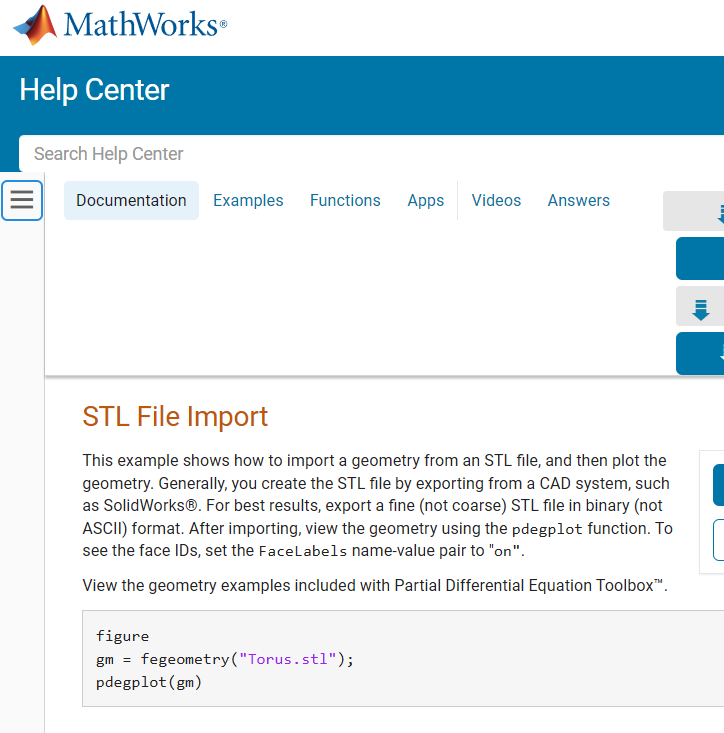
\includegraphics[width=2.0in ]{pics/stl.png}
  \caption{stl file import into MATLAB\textsuperscript{\textregistered}.}
  \label{stl}
\end{figure}



So we would have to obtain the robot's CAD models from the manufacturer's website, then edit them on a 3D CAD Software into individual parts. This is because MATLAB\textsuperscript{\textregistered} reads the .stl files for each link separately. The 3D model of the ABB 120 was found online but it was an assembly which was in .step format. I converted the individual parts into stl format and was using the SolidWorks' Move and Rotate feature to orient the link's origin so as it was consistent with the Denavit Hartenberg model (stick figure) we constructed earlier on MATLAB. I also had to scale down the modles by 1000 since the Robotics Toolbox uses metres as opposed to millimetres on SolidWorks. It is also important to note that upon reading on the book \textit{Robotics Toolbox for MATLAB} by Peter Corke, he specified the package ARTE by Arturo Gil \cite{ARTEARob24:online} which had already included the 3D models of some robots in the Robotics Toolbox (version 10.4), including the ABB IRB 120. The task would be as simple as downloading the stl files from ARTE's library \cite{ARTEARob24:online} and calling the function \texttt{Serialplot3D()}, while specifying the parameters.


\begin{figure}[H]
  \centering
  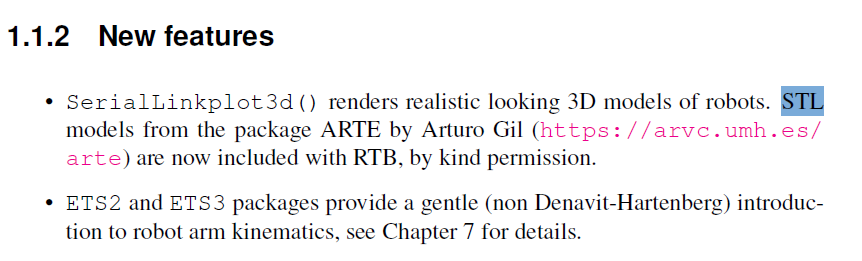
\includegraphics[width=3.0in ]{pics/Screenshot_7.png}
  \caption{ARTE package by Arturo Gil \cite{RoboticsToolbox}}
  \label{arte}
\end{figure}


The 3D model simulation can be seen on the below image:


\begin{figure}[H]
  \centering
  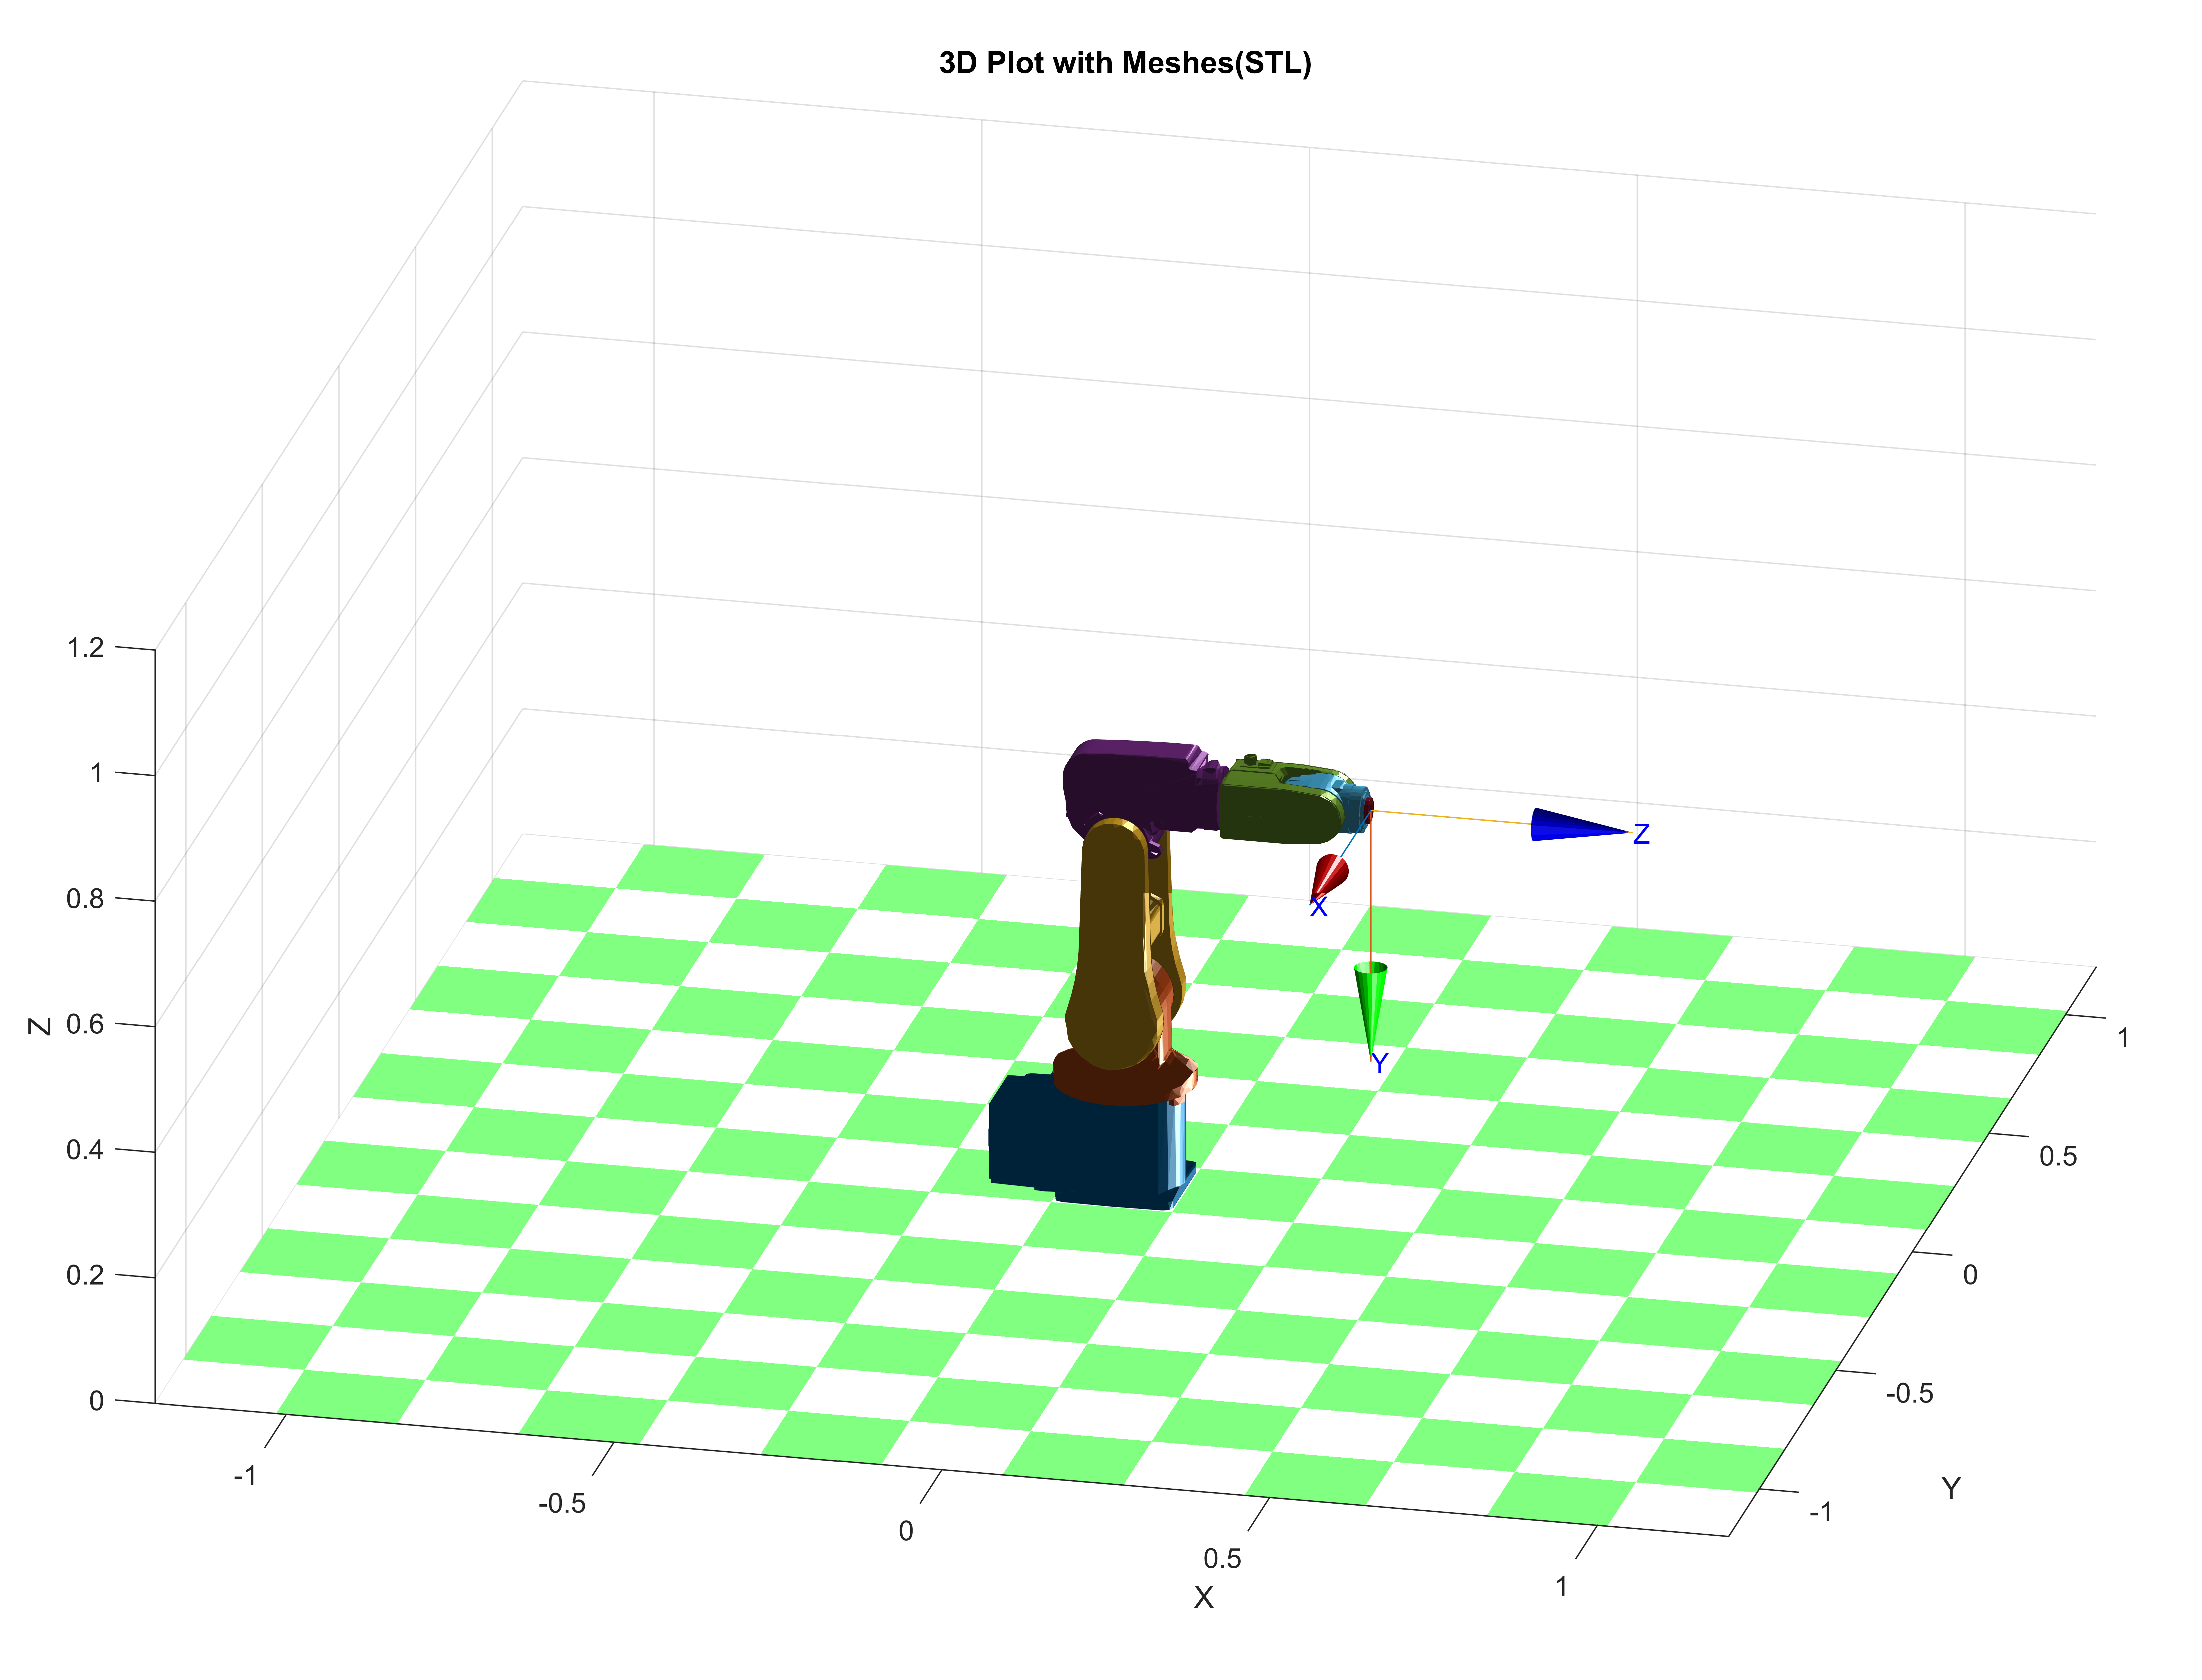
\includegraphics[width=3.6in ]{pics/3d stl.png}
  \caption{3D CAD Model Visualization on RTB}
  \label{3d}
\end{figure}



\subsection{Challenges encountered during 3D model animation}
After successfully importing the 3D model of the robot into MATLAB, we tried to
move the same way as the physical robot in the pick and place task. The image
coordinates were to be obtained from the Image Recognition code and then input
into the inverse kinematics solution. These inputs are three coordinates which is
the image x, y and its orientation. 

\noindent Unfortunately, this posed a challenge as our inverse kinematics solution failed to address this 
matter. To generate the appropriate joint angles, the inverse kinematics solution
required the image / object's x, y and z coordinates in 3d vector matrix as well
as its orientation (px, py and pz). The inverse kinematics solution totally failed
to address this issue and thus we could not animate the robot as based on the 
image coordinates. A suggestion was put that the image coordinates to be converted
to 3d vector format and since the z coordinate is already known, then this would 
be input to the inverse kinematic solution. Further research and understanding needs to be done in 
this area and appropriate solution needs to be done especially when calculating 
inverse of a six degrees of freedom robot using the analytical way. 





\section{Conclusion}
This project successfully demonstrates a robust method for integrating \texttt{MATLAB\textsuperscript{\textregistered}} and \texttt{RAPID} for pick and place operations using socket communication. The \texttt{RAPID} program efficiently handles the data received from \texttt{MATLAB\textsuperscript{\textregistered}}, sorts the objects based on a property value, and performs the pick and place operations to stack it at the \texttt{stackPoint} to form a pyramid structure. The
integration between \texttt{MATLAB\textsuperscript{\textregistered}} and the \texttt{ABB} robot controller through socket communication enables efficient and precise control of the robot arm for pick and place tasks based on real-time data from image processing. This setup can be adapted and extended for various industrial applications involving robotic automation. 
By implementing the kinematic decoupling approach, the inverse kinematics problem for the ABB IRB 120 robot can be solved, making it able to control of the robot's end-effector position and orientation.





\section*{Appendix}
\large\href{https://studentsswinburneedu-my.sharepoint.com/:f:/g/personal/101229220_students_swinburne_edu_my/EtwPYa2U7ctPskWgIqP-EhEBreegVWK0ACHmneuZSLz_TQ?e=V1dBor}{Link to Code files}

